\documentclass[a4paper,12pt]{article}

\usepackage{geometry}
\usepackage{polski}
\usepackage{amsmath}
\usepackage{ragged2e}
\usepackage{graphicx}
\usepackage{xcolor}
\usepackage{siunitx}
\usepackage{multirow}
\usepackage{pdfpages}
\usepackage{listings}

\graphicspath{ {./img/} }

\newcommand\crule[3][black]{\textcolor{#1}{\rule{#2}{#3}}}

\geometry{
 a4paper,
 total={170mm,257mm},
 left=20mm,
 top=20mm,
 }

\definecolor{amethyst}{rgb}{0.6, 0.4, 0.8}

\begin{document}
\title{Systemy równoległe i rozproszone - Klasyfikator dokumentów (UPC++)}
\author{Piotr Moszkowicz} 
\date{\today}
\maketitle
\pagenumbering{roman}

\newpage
\begin{justify}
\tableofcontents
\newpage
\pagenumbering{arabic}

\section{Wstęp}

W ramach drugiego projektu jego celem było zaprojektowanie współbieżnego programu z wykorzystaniem technologii PGAS zaimplementowanej w języku UPC++, który mógłby klasyfikować dokumenty.

\subsection{Problem klasyfikacji}

W tym wypadku klasyfikowane były pliki tekstowe formatów .html, .txt oraz .tex. Klasyfikacja odbywa się na podstawie pliku słownika $dict.txt$. W tym pliku znajdują się słowa kluczowe, które wyszukujemy we wszystkich pozostałych plikach w katalogu spełniających kryterium formatu. Następnie zliczana jest ilość słów w tych plikach, a finalnie rezultat jest sumowany.

\section{Budowa programu}

Program opiera się o mechanizm Manager - Workers. Jest to implementacja szeroko znanego wzorca map-reduce, wykorzystywanego między innymi w środowisku Spark. Procesowi zerowemu przypisujemy rolę managera zadań, którego zadaniem jest wczytanie listy dostępnych plików, a następnie rozdysponowanie ich pomiędzy workery. Zadaniem workerów jest policzenie słów w danym pliku (operacja "map"). Manager ma dodatkową rolę - na początku działania aplikacji jego zdaniem jest wczytanie słownika oraz przesłanie go do pozostałych workerów, które w ramach swojej dostępnej pamięci tworzą jego kopię w celu posiadania wiedzy jakie słowa kluczowe są poszukiwane. Sama implementacja wyszukiwania jest trywialna - zadany plik jest otwierany, a następnie słowo po słowie liczone są jego wyrazy. Finalnie z mapy wystąpień wyrazów wybieramy tylko te, które nas interesują. Gdy rezultaty z wszystkich procesów zostaną dostarczone managerowi ten wykonuje operację "reduce" - sumuje wystąpienia we wszystkich plikach i zapisuje wyniki do pliku wynikowego $result.txt$. 

\pagebreak

\begin{figure}[h!]
\centering
\frame{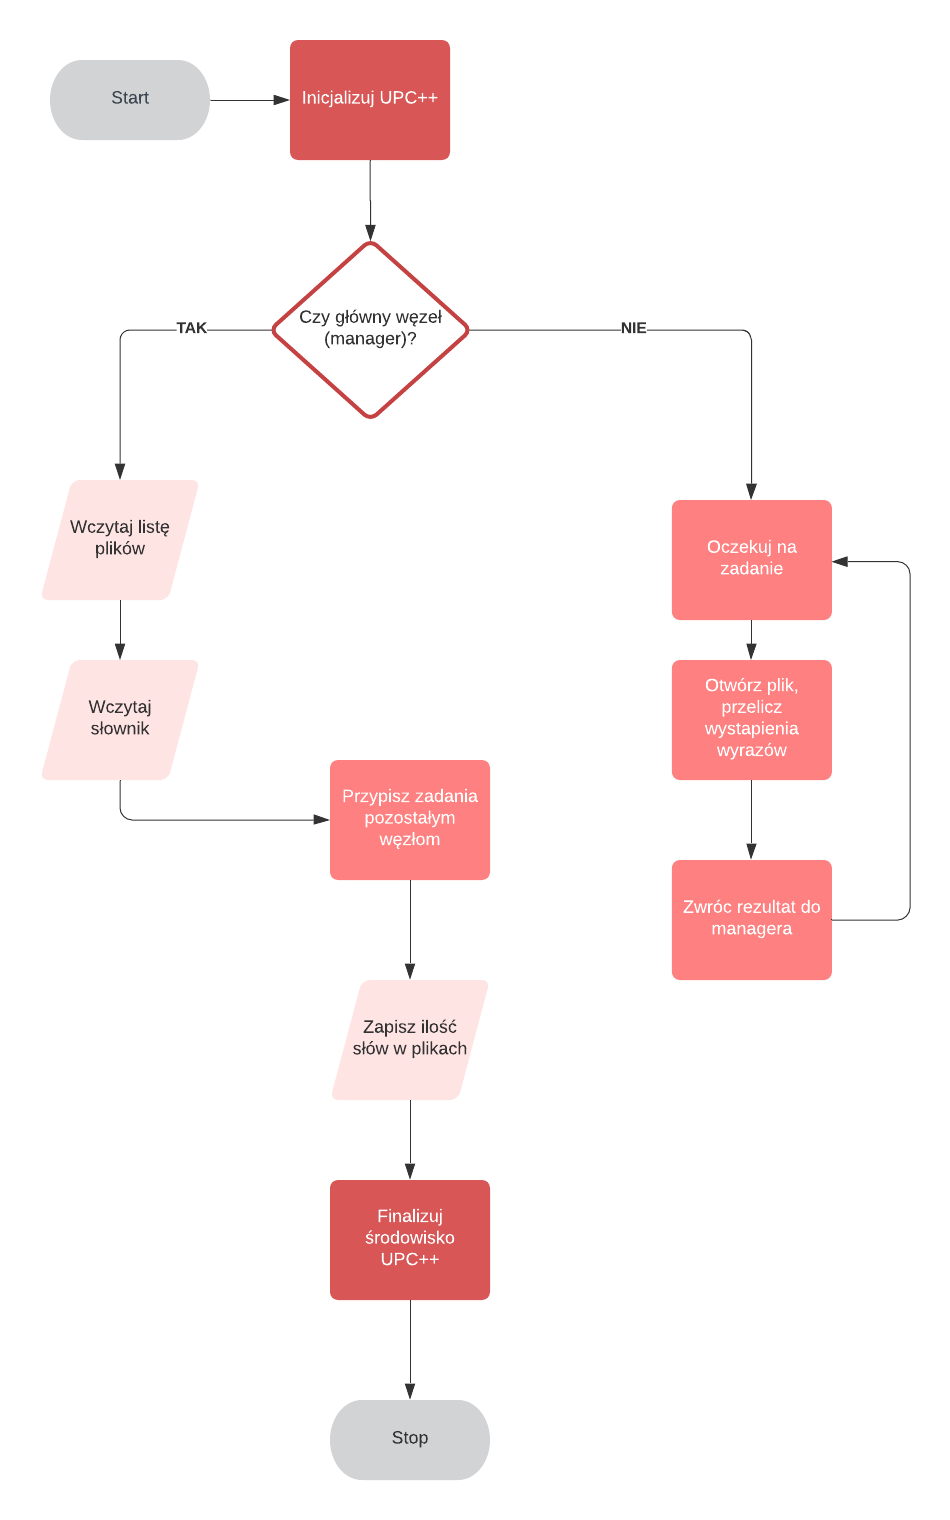
\includegraphics[width=18cm,height=24cm]{MPI_Proj_Flow_2}}
    \caption{Schemat blokowy programu}
\end{figure}

\pagebreak

Sam program został napisany w języki C++ w standardzie C++17 (głównie ze względu na nagłówek $filesystem$). Wersja środowiska UPC++ to 2021.3.0. Z ciekawostek - zastosowano funkcjonalność "Conjoining Futures", która pozwala na równoczesne zlecenie wszystkich zadań swoiście dokładając je do siebie (mimo tego, iż wykonywane są na różnych węzłach). Finalnie główny proces oczekuje na wykonanie wszystkich zadań, a nie na każde po kolei. Dzięki temu program faktycznie jest asynchroniczny. Aby rezultaty mogły być poprawnie zapisane należało zmienić strukturę danych rezultatu - każdy worker zwraca $std::pair<std::string, std::vector<int>>$, gdzie pierwszym elementem pary jest nazwa pliku, natomiast drugi wektor wyrazów (słownik ma tę samą kolejność dla każdego workera, więc sam vector wystarczy).

\section{Obsługa programu}

Wraz z programem zostały dostarczone przykładowe pliki wejściowe oraz plik $makefile$, który pozwala na kompilację oraz uruchomienie programu. Procedura $make compile$ kompiluje program, a z pomocą procedury $make run$ możemy uruchomić program (domyślnie na 8 węzłach). Przed tym należy jednak skonfigurować środowisko UPC++ wykorzystując skrypty dostępne na serwerze Taurus.

Dla przykładowych danych testowych (umieszczonych w archiwum) osiągnięto następujący rezultat: \\
$
7moszkowicz@stud206-001:~/WFiIS-SRiR-2021/proj2\$ cat result.txt \\
1 \\
1 \\
2 \\
$

\end{justify}
\end{document}